\documentclass[a4paper]{article}
\linespread{1.5}
\usepackage[round]{natbib}
\usepackage{amssymb}
%% \usepackage{RJournal}
\usepackage{fancyvrb}
\usepackage{Sweave, url, tikz}
\usepackage{hyperref}
\usepackage[sc]{mathpazo}
\usepackage[T1]{fontenc}
\usepackage{geometry}
\geometry{verbose,tmargin=2.5cm,bmargin=2.5cm,lmargin=2.5cm,rmargin=2.5cm}
\setcounter{secnumdepth}{2}
\setcounter{tocdepth}{2}
\usepackage{url}
\usepackage{breakurl}
\usepackage[utf8]{inputenc}

\newcommand{\ts}{\textsuperscript}
\newcommand\bc{\begin{center}}
\newcommand\ec{\end{center}}



\bibliographystyle{abbrvnat}

\begin{document}
\title{A Guide to the CDS Package (Draft)}
\author{Heidi Chen\thanks{\href{mailto:s.heidi.chen@gmail.com}{s.heidi.chen@gmail.com}}, David Kane\thanks{\href{mailto:dave.kane@gmail.com}{dave.kane@gmail.com}}, and Yang Lu\thanks{\href{mailto:yang.lu2014@gmail.com}{yang.lu2014@gmail.com}}}
\maketitle

%%\VignetteIndexEntry{Using the CDS package}
%%\VignetteDepends{CDS}

%% \setkeys{Gin}{width=0.95\textwidth}


\section{Introduction}

%% 1 paragraph

A Credit Default Swap (CDS) is a financial swap agreement between two
counterparties in which the buyer pays a fixed periodic coupon to the
seller in exchange for protection in the case of a credit event. The
International Swaps and Derivatives Association (ISDA) has created a
set of standard terms for CDS contracts, the so-called ``Standard
Model.'' This allows market participants to calculate cash settlement
from conventional spread quotations, convert between conventional
spread and upfront payments, and build the yield curve of a CDS. The
\textbf{CDS} package implements the Standard Model, allowing users to
value credit default swaps and calculate various risk measures
associated with these instruments.

\section{CDS Basics}


%% what's a CDS

A CDS is a simple and popular form of credit derivative. It was
originated in the late 1980s and was popularized by a team at
J.P. Morgan including Blythe Masters in 1994 \citep{cdsOrigins,
  blythe}. The CDS market started to develop soon afterwards as banks
used CDS contracts to hedge their credit exposures on the balance
sheets. Many different types of CDS have since emerged including
basket default swaps (BDSs), index CDSs, credit-linked notes, et
cetera \citep{jk}. In the \textbf{CDS} package, we focus on calculations
related to a single-name CDS contract.

%% mechanics of a single-name CDS contract

A single-name CDS contract provides a transfer of credit risk between
two parties. The buyer of a CDS contract, a.k.a. protection buyer,
transfers the credit risk to the CDS seller (or called protection
seller) by paying a series of payments before the contract
terminates. In other words, the protection buyer is short credit by
selling the credit risk of an underlying loan to the protection
seller. As shown in Figure \ref{fig:cashFlow}, the buyer pays a stream
of coupon payments, called the premium leg, in order to receive a
one-off, contingent payment (protection leg) in the case of a credit
event.\\

%% add a diagram on buyer and seller of CDS?

\begin{figure}
  \caption{\label{fig:cashFlow} Mechanics of a CDS contract}
\begin{center}
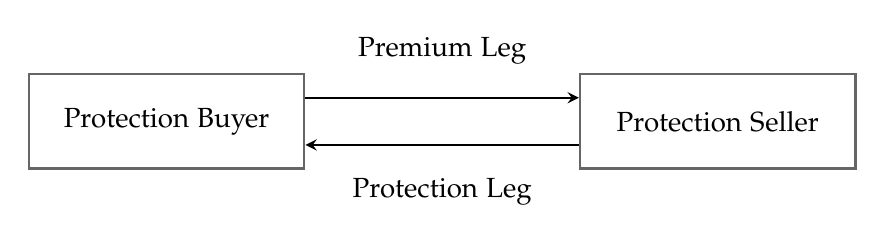
\begin{tikzpicture}[
squarednode/.style={rectangle, draw=black!60, fill=none, thick, 
  minimum height =12mm, minimum width = 35mm},
]
  \tikzset{mylabel/.style = {text centered}
  }

\vspace{2cm}
    \node [squarednode](A) at (0,0) {Protection Buyer};
    \node [squarednode](B) at (7,0) {Protection Seller};

    \draw[transform canvas={yshift=3mm},-stealth, thick] (A) -- (B);
    \draw[transform canvas={yshift=-3mm},-stealth, thick] (B) -- (A);
    \node[mylabel] at (3.5, 0.9) {Premium Leg};
    \node[mylabel] at (3.5, -0.9) {Protection Leg};
    
\end{tikzpicture} 
\end{center}
\end{figure}

In the package \textbf{CDS}, we call the function \texttt{CDS} to construct an object of a class ``CDS''. Below we show an example of a CDS contract.


\begin{Schunk}
\begin{Sinput}
> library(CDS)
> cds1 <- CDS(entityName = "IBM",
+             RED = "49EB20",
+             TDate = "2014-04-15",
+             maturity = "5Y",
+             notional = 1e7,
+             coupon = 100,
+             parSpread = 50)
\end{Sinput}
\end{Schunk}

A CDS contract between two counterparties typically specifies the
following key terms:\footnote{Some of the definitions come from
  \textit{Credit Derivatives Glossary} \citep{glossary},
  \textit{Standard Corporate CDS Handbook} \citep{barclays},
  \textit{Credit Derivatives} \citep{bloomberg}, and \textit{The
    Pricing and Risk Management of Credit Default Swaps, with a Focus
    on the ISDA Model} \citep{openGamma}.}
\begin{description}
\item[Reference Entity] refers to the legal entity which is the
  subject of a CDS contract. 
\item[Notional] is the amount of the underlying asset on which the
  payments are based.
\item[Maturity] a.k.a \textbf{tenor}. It refers to the length of a CDS
  contract. Most CDSs are written with 5 years of maturity. The
  protection buyer continues to make payments to the protection seller
  till maturity of the contract or the occurrence of a credit event.
\item[Coupon] is often quoted in basis points. It specifies the
  payment amount from the protection buyer to the seller on a regular
  basis.
\item [Premium Leg] refers to the cashflows of the fixed payments made
  by the protection buyer.
\item [Contingent Leg], a.k.a. \textbf{protection leg}, is the payment
  of notional less recovery amount by the protection seller after a
  credit event.
\item[Par Spread] is quoted in basis points per annum. It represents
  the fair rate for a contract of 1 year beginning on the trade date.
\item[Seniority] specifies the order of which the debt will be paid in
  liquidation or bankruptcy. In general, there are four levels of
  seniority - Senior, Subordinated, Junior, and Preferred.
\item[Credit Event] triggers the settlement under a CDS
  contract. Possible credit events specified by the ISDA Credit
  Derivatives Definitions include: 
  \begin{itemize}
  \item Bankruptcy - It typically occurs when the reference entity has
    filed under a bankruptcy law (or an equivalent law).
  \item Failure to pay - The reference entity fails to make interest
    or principal payments when due after the applicable grace period
    expires.
  \item Debt restructuring - The specifications of the debt
    obligations are changed such that the protection buyer is
    unfavorably affected.
  \item Obligation acceleration - A debt obligation becomes due before
    it would otherwise have been because of a default.
  \item Obligation default - A debt obligation becomes capable of
    being declared due before it would otherwise have been because of
    a default.
  \item Repudiation/Moratorium - The reference entity announces
    repudiation or moratorium on debt obligation and subsequently
    fails to pay.
  \end{itemize}
\end{description}

\section{The ISDA Standard Model}

%% the origins of the ISDA standard model
In April 2009 in North America and June 2009 in Europe, the ISDA
introduced a series of mandatory modifications to the CDS contract
known as the ``Big Bang Protocol.'' Among these changes were the
standardization rules on the first accrual dates, fixed coupon rates
(100 bps or 500 bps), and the recovery rate (40 \%).

%% specifications of the ISDA standard CDS contract
The default calculations and parameters in the \textbf{CDS} package
follow the Standard Model. The user can call \texttt{summary} on a
``CDS'' class object to view essential information on the contract
(including trade date, maturity date, spread, and coupon rate as
specified by the user) and some relevant calculations based on the
input CDS contract and the ISDA standard calculations.

\begin{Schunk}
\begin{Sinput}
> cds1 <- CDS(entityName = "IBM",
+             RED = "49EB20",
+             TDate = "2014-04-15",
+             maturity = "5Y",
+             notional = 1e7,
+             coupon = 100,
+             parSpread = 50)
> summary(cds1)
\end{Sinput}
\begin{Soutput}
Contract Type:                      SNAC   TDate:                     2014-04-15
Entity Name:                         IBM   RED:                           49EB20
Currency:                            USD   End Date:                  2019-06-20
Spread:                               50   Coupon:                           100
Upfront:                        -256,577   Spread DV01:                    5,086
IR DV01:                           66.14   Rec Risk (1 pct):               90.03
\end{Soutput}
\end{Schunk}


%% This section provides some key specifications of the ISDA Standard
%% Model.\footnote{Refer to the \textit{ISDA Standard CDS Converter
%%     Specification} for details.} The default calculations and
%% parameters in the \textbf{CDS} package follow the Standard
%% Model. Additional default settings in the package which are not
%% specified by the Standard Model, such as the default notional amount,
%% are also listed.

The \texttt{summary} information reflects the key specifications of
the ISDA Standard Model explained in this section.\footnote{Refer to
  the \textit{ISDA Standard CDS Converter Specification} for details.}


\subsection{Standard Model Specifications}
An ISDA standard CDS contract specifies the following:
\begin{description}
\item [Trade Date] refers to the date of the trade.
\item [Maturity] is the length of the contract. Most of the standard
  contracts have a maturity of 5 years.
\item [Maturity Date] falls on one of the four dates (Mar/Jun/Sep/Dec
  20th) in a year. One can add the maturity of the contract to the
  trade date; the next available date among those four dates is the
  maturity date.
\item [Backstop Date] is the date from which protection is
  provided,
  \begin{center}
    Backstop Date = T - 60 Calender Days.
  \end{center}
\item [Notional Amount] is denoted in millions.
\item [Standard Coupon] is quoted either 100 bps or 500 bps per
  annum for CDS contracts in North America, and 25 bps, 100 bps, 500
  bps or 1000 bps in Europe.
\item [Recovery Rate] is the estimated percentage of par value that
  bondholders will receive after a credit event. It is commonly
  reported in percentages. A CDS contract for investment grade bonds
  are assumed a 40\% recovery rate when it is valued. The recovery
  rate is assumed to be 20\% when valuing a subordinate level
  CDS. 25\% is assumed for emerging markets' CDSs (both senior and
  subordinate).
\item [Par Spread] is the spread value which makes the present value
  of a CDS contract zero. It is quoted in basis points.  
\item [Upfront Payment] is quoted in the currency amount. Since a
  standard contract is traded with fixed coupons, upfront payment is
  introduced to reconcile the difference in contract value due to the
  difference between the fixed coupon and the conventional par
  spread. There are two types of upfront, dirty and clean. Dirty
  upfront, a.k.a. \textbf{Cash Settlement Amount} refers to the market
  value of a CDS contract. Clean upfront is dirty upfront less any
  accrued interest payment, and is also called the \textbf{Principal}.
\item [Points Upfront], or simply \textbf{points}, are quoted as a
  percentage of the notional amount. They represent the upfront
  payment excluding the accrual payment. High Yield (HY) CDS contracts
  are often quoted in points upfront. The protection buyer pays the
  upfront payment if points upfront are positive, and the buyer is
  paid by the seller if the points are negative.
\end{description}

\subsection{Standard Model Pricing}
\label{sec:pricing}
The Standard Model allows market participants to convert between
the par spread and the upfront payment, and compute the cash
settlement amount for a standard contract. A few key assumptions and
definitions used when valuing a Standard CDS contract are the
following:\footnote{Please refer to \url{http://bit.ly/1kg5qPw} for
  more infrmation on the ISDA standard CDS model assumptions.}

%% cds converter specification pdf original
%% url. http://www.cdsmodel.com/assets/cds-model/docs/ISDA\%20Standard\%20CDS\%20Contract\%20Converter\%20Specification\%20-\%20Sept\%204,\%202009.pdf}

\begin{description}
\item [Trade Date (T)] means 11:59pm on the trade date.
\item [Days of Protection] are the difference in the number of days
  from Maturity Date to Trade Date.
\item [Mark-to-market (MTM)] represents the contract value to the
  protection buyer. It is computed by discounting the expected
  protection leg and premium leg cashflows to T.
\item [Accrued Premium] is the premium that has accrued from accrual
  begin date to T where both dates are inclusive.
\end{description}

%% http://www.cdsmodel.com/assets/cds-model/docs/Interest%20Rate%20Curve%20Specification%20-%20All%20Currencies%20%28Updated%20May%202013%29.pdf


The ISDA also standardizes the interest rates used by the Standard
Model in valuting a CDS contract. There are two types of rates used in
valuing a USD denominated CDS contract - cash rates and swap
rates. Cash rates are of maturity 1, 2, 3, 6 months, and 1 year. They
are provided by the British Bankers' Association (BBA). Swap rates are
of maturity 2, 3, 4, 5, 6, 7, 8, 9, 10, 12, 15, 20, 25, 30 years and
are provided by ICAP \citep{rates}. The Standard Model follows the
conventions below for interpolation of the entire USD yield
curve:
\begin{itemize}
\item The day count convention (DCC) for money market instruments and
  floating legs of the swaps is \textbf{ACT/360}.
\item DCC for floating legs of the swaps is \textbf{30/360}.
\item Payment frequency for fixed legs of the swaps is 6 months.
\item Payment frequency for floating legs of the swaps is 3
  months.\footnote{See
    \url{http://www.fincad.com/derivatives-resources/wiki/swap-pricing.aspx}
    for details on floating and fixed legs calculation.}
\item A business day calendar of weekdays (Monday to Friday) is
  assumed. Saturdays and Sundays will be the only non-business days.
\item If a date falls on a non-business day, the convention used for
  adjusting coupon payment dates is \textbf{M} (Modified Following).
\end{itemize}

One component essential to the mark-to-market calculation of a CDS
contract is \textbf{PV01}. It is the present value of a stream of 1
basis point payments at each CDS coupon date. It is sometimes referred
to as the \textbf{CDS duration} or \textbf{risky duration}.

Analytically, PV01 can be calculated by
\begin{displaymath}
PV01 =  \sum_tDf(t_i)S(t_i)B(t_i), \nonumber\\
\end{displaymath}
where 
\begin{itemize}
\item $i =$ coupon index,
\item $t_i =$ coupon date,
\item $Df(f_i) =$ discount factor until $t_i$,
\item $S(t_i) =$ survival probability until $t_i$,
\item $B(t_i) =$ day count fraction at $t_i$.
\end{itemize}

We can thus calculate the principal amount (clean upfront payment)
paid from the protection buyer to the seller using the following
formula:
\begin{center}
  Principal Amount = (Par Spread - Coupon) $\times$ PV01.
\end{center}

Using the concept of PV01, we show the calculation of the main risks
(exposures) of a CDS position, \textbf{Spread DV01}. Spread DV01
reflects the risk duration of a CDS trade, also known as \textbf{Sprd
  DV01}, \textbf{Credit DV01}, \textbf{Spread Delta}, and just
\textbf{DV01}. 
%% It is the sensitivity of the CDS contract to a parallel
%% shift in the CDS spreads.  
It measures the sensitivity of a CDS contract mark-to-market to a
parallel shift in the term structure of the par spread. DV01 should
always be positive for a protection buyer since she is short credit
and a rising spread is a sign of credit deterioration. Starting with
PV01 and taking the derivative with respect to the spread give us:
\begin{eqnarray}
  PV & = & (S - C) * PV01 \nonumber \\
  DV01 & = & \frac{\partial PV}{\partial S} \nonumber \\
  & = & PV01 + (S - C) \frac{\partial PV01}{\partial S},\nonumber
\end{eqnarray}
where $S$ is the spread of the contract and $C$ is the coupon.

Both DV01 and PV01 are measured in dollars and are equal if the spread
equals the coupon. 

%% In other words, the relationship between spread (on
%% the x-axis) and dollars (on the y-axis) is identical when the spread
%% is equal to the coupon. That is where these two lines cross. 

%% DV01 will be great than PV01 when spread is greater than coupon, I
%% guess.

Some other risk measures of a CDS contract are as follows:
\begin{description}
\item[IR DV01] is the change in value of a CDS contract for a 1 bp
  parallel increase in the interest rate curve. IR DV01 is, typically,
  a much smaller dollar value than Spread DV01 because moves in
  overall interest rates have a much smaller effect on the value of a
  CDS contract than does a move in the CDS spread itself.
%% \item [Spread DV01], aka spread delta, measures the sensitivity of a
%%   CDS contract MTM to a parallel shift in the term structure of the
%%   par spread. Spread DV01 in Bloomberg is, typically, a much larger
%%   dollar value than IR DV01 because moves in overall interest rates
%%   have a much smaller effect on CDS value than does a move in the CDS
%%   spread itself.
\item [Recovery Risk 01] is the dollar value change in market value if
  the recovery rate used in the CDS valuation were increased by 1\%.
\item[Price] refers to the clean dollar price of the contract. 
  \begin{eqnarray}
    {\rm Price} & = & (1 - {\rm Principal} / {\rm Notional})*100  \nonumber \\
    & = & 100 - {\rm points upfront}. \nonumber
  \end{eqnarray}
  For example, if a CDS contract is quoted as 3 points to buy
  protection, the price will be 97. The protection buyer still pays
  the 3\% as an upfront fee. A CDS will have a price greater than 100
  if the points upfront are negative, that is, the CDS buyer needs to
  receive money to obtain protection because he promises to pay a
  coupon of, say, 100 even if the spread is 60. This is analogous to a
  bond investor paying more than the face value of a bond because
  current interest rates are lower than the coupon rate on the bond.
\end{description}


\section{Using the CDS package}
Currently, a market participant can conduct CDS-related calculations
by using the \textbf{CDSW Calculator} on a Bloomberg Terminal or the
Markit CDS Calculator.\footnote{The Markit CDS Calculator is available
  at \url{http://www.markit.com/markit.jsp?jsppage=pv.jsp}.} The
\textbf{CDS} package provides tools for valuing a single-name CDS
contract. The default setting allows a user to value a USD-denominated
CDS contract following the Standard Model. She can also specify her
own set of parameters to customize the calculation. We have
illustrated the construction of a CDS contract using the \textbf{CDS}
package in previous sections. In this section, we will demonstrate the
use of the \textbf{CDS} package in more detail and provide a series of
examples.

The default settings of valuing a CDS contract in the \textbf{CDS}
package follow the Standard North American Corporate (SNAC) CDS
Contract specifications.\footnote{See
  \url{http://www.cdsmodel.com/assets/cds-model/docs/Standard\%20CDS\%20Contract\%20Specification.pdf}
  for details.} Below we list the ISDA specifications implemented in
the \textbf{CDS} package. Additional default settings in the package
which are not specified by the Standard Model, such as the default
notional amount, are also listed.


\begin{itemize}
\item Currency: USD.
\item Trade Date (T): the current business day.
\item CDS Date: Mar/Jun/Sep/Dec 20th of a year.
\item Maturity: 5 years.
\item Maturity Date (End Date): It falls on a CDS date without
  adjustment.
\item Coupon Rate: 100 bps.
\item Notional Amount (MM): 10MM.
\item Recovery Rate (\%): 40\% for senior debts.
\item Premium Leg:
  \begin{itemize}
    \item Payment Frequency: quarterly
    \item DCC: ACT/360
    \item Pay Accrued On Default: It determines whether accrued
      interest is paid on a default. If a company defaults between
      payment dates, there is a certain amount of accrued payment that
      is owed to the protection seller. ``True'' means that this
      accrued will need to be paid by the protection buyer, ``False''
      otherwise. The defalt is ``True,''
    \item Adjusted CDS Dates: ``F''. It means that it assumes the next
      available business day when a CDS date falls on a non-business day
      except the maturity date.
    \item First Coupon Payment: It is the earliest Adjusted CDS Date
      after T + 1.
    \item Accrual Begin Date (Start Date): It is the latest Adjusted
      CDS Date on or before T + 1.
    \item Accrual Period: It is from previous accrual date (inclusive)
      to the next accrual date (exclusive), except for the last
      accrual period where the accrual end date (Maturity Date) is
      included.
  \end{itemize}
\item Protection Leg:
  \begin{itemize}
  \item Protection Effective Date (Backdrop Date): T - 60 calendar
    days for credit events.
  \item Protection Maturity Date: Maturity Date.
  \item Protection Payoff: Par minus Recovery.
  \end{itemize}
\end{itemize}


For the example we have shown in the previous sections,

\begin{Schunk}
\begin{Sinput}
> library(CDS)
> cds1 <- CDS(entityName = "IBM",
+             RED = "49EB20",
+             TDate = "2014-04-15",
+             maturity = "5Y",
+             notional = 1e7,
+             coupon = 100,
+             parSpread = 50)
\end{Sinput}
\end{Schunk}

\texttt{entityName} indicates the name of the underlying entity which
is the subject of the CDS contract. \texttt{RED} is a Markit
product. It stands for Reference Entity Database. Each
entity/seniority pair has a unique 6 digit RED code. Each deliverable
bond has a 9 digit RED code, the first 6 digits of which matches the 6
digit code of the associated entity/seniority. Each entity also has a
``preferred reference obligation'' that is the default reference
obligation for CDS trades. A user can input either the six-digit RED
code or the nine-digit RED pair code. \texttt{TDate} indicates the
trade date of the CDS contract. \texttt{maturity} is the maturity of
the contract. \texttt{coupon} is the fixed coupon of the
contract. \texttt{parSpread}, \texttt{ptsUpfront} and \texttt{upfront}
refer to the par spread (in bps), points upfront (in \%), and upfront
payment (in dollar amount) of a CDS contract, respectively. One of the
three arguments has to be specified in order to construct the ``CDS''
class object.

Here the user has entered the CDS contract which has ``IBM'' as the
underlying entity with ``49EB20'' as the RED Code. She sets the spread
at 50 bps and the coupon rate at 100 bps. However, the valuation of a
CDS contract requires neither the entity name or the RED Code. She
does not have to know the information to use the package. As shown
below, insofar as she inputs the same \texttt{TDate},
\texttt{parSpread}, and \texttt{maturity} information, the valuation
of the contract will be the same.

\begin{Schunk}
\begin{Sinput}
> cds2 <- CDS(TDate = "2014-04-15",
+             maturity = "5Y",
+             coupon = 100,
+             parSpread = 50)
\end{Sinput}
\end{Schunk}

%% Calling \texttt{summary} on a ``CDS'' class object provides some
%% essential information on the contract (including trade date, maturity
%% date, spread, and coupon rate as specified by the user) and some
%% relevant calculations based on the input CDS contract.

Calling \texttt{summary} on the two CDS contracts provides the same information.

\begin{Schunk}
\begin{Sinput}
> summary(cds1)
\end{Sinput}
\begin{Soutput}
Contract Type:                      SNAC   TDate:                     2014-04-15
Entity Name:                         IBM   RED:                           49EB20
Currency:                            USD   End Date:                  2019-06-20
Spread:                               50   Coupon:                           100
Upfront:                        -256,577   Spread DV01:                    5,086
IR DV01:                           66.14   Rec Risk (1 pct):               90.03
\end{Soutput}
\begin{Sinput}
> summary(cds2)
\end{Sinput}
\begin{Soutput}
Contract Type:                      SNAC   TDate:                     2014-04-15
Entity Name:                          NA   RED:                               NA
Currency:                            USD   End Date:                  2019-06-20
Spread:                               50   Coupon:                           100
Upfront:                        -256,577   Spread DV01:                    5,086
IR DV01:                           66.14   Rec Risk (1 pct):               90.03
\end{Soutput}
\end{Schunk}

In the \texttt{summary} output, \texttt{Upfront} shows the cash
settlement amount (dirty upfront). It is the sum of the principal and
the accrual. \texttt{Spread DV01}, \texttt{IR DV01}, and \texttt{Rec
  Risk (1 pct)} are the eponymous results mentioned in Section
\ref{sec:pricing}. Moreover, \texttt{summary(cds1)} and
\texttt{summary(cds2)} give the same output besides
\texttt{entityName} and \texttt{RED}. 

\begin{Schunk}
\begin{Sinput}
> cds2.CS10 <- CS10(cds2)
> cds2.CS10
\end{Sinput}
\begin{Soutput}
[1] 25385.2
\end{Soutput}
\end{Schunk}

\texttt{CS10} is a method which calculates the change in value of the
CDS contract when the spread of the contract increases by
10\%. \texttt{CS10} takes in a \texttt{CDS} class object formed by
calling the \texttt{CDS} function.

\begin{Schunk}
\begin{Sinput}
> cds3 <- update(cds1, spread = 55)
\end{Sinput}
\end{Schunk}

The \texttt{update} method updates a ``CDS'' class object with a new
spread, points upfront or upfront by specifiying the relevant
input. \texttt{cds3} is a new ``CDS'' class object with a spread of 52
bps; all other specifications of the contract are the same as those in
\texttt{cds1} since it is updated from \texttt{cds1}. One can also
specify \texttt{upfront} (in dollar amount) or \texttt{ptsUpfront} (in
bps) in the \texttt{update} method.

Besides calling the \texttt{summary} method, one can type in the name
of the ``CDS'' class object in the current \textbf{R} Session and
obtain a full description of the CDS contract.

\begin{Schunk}
\begin{Sinput}
> cds3
\end{Sinput}
\begin{Soutput}
CDS Contract 
Contract Type:                      SNAC   Currency:                         USD
Entity Name:                         IBM   RED:                           49EB20
TDate:                        2014-04-15   End Date:                  2019-06-20
Start Date:                   2014-03-20   Backstop Date:             2014-02-14
1st Coupon:                   2014-06-20   Pen Coupon:                2019-03-20
Day Cnt:                         ACT/360   Freq:                               Q

Calculation 
Value Date:                   2014-04-18   Price:                         102.24
Spread:                               55   Pts Upfront:                  -0.0224
Principal:                      -223,692   Spread DV01:                    5,064
Accrual:                          -7,500   IR DV01:                        59.35
Upfront:                        -231,192   Rec Risk (1 pct):               88.87
Default Prob:                      0.047   Default Expo:               6,223,692

Credit curve effective of2014-04-15 
 Term     Rate Term     Rate
   1M 0.001517   7Y 0.022630
   2M 0.001923   8Y 0.024580
   3M 0.002287   9Y 0.026265
   6M 0.003227  10Y 0.027590
   1Y 0.005465  12Y 0.029715
   2Y 0.005105  15Y 0.031820
   3Y 0.009265  20Y 0.033635
   4Y 0.013470  25Y 0.034420
   5Y 0.017150  30Y 0.034780
   6Y 0.020160              
\end{Soutput}
\end{Schunk}

There are three parts of the output. They are the basic contract
information, the valuation of the contract, and the interest rates
used in the calculation.

Calling the function \texttt{getRates} produces the rates used in
building a curve for CDS valuation. 

\begin{Schunk}
\begin{Sinput}
> cds1Rates <- getRates(date = "2014-01-15")
\end{Sinput}
\end{Schunk}

The output consists of two list objects. The first list contains rates
of various maturities. They are directly obtained from the Markit
website based on the specifications \citep{rates}.

\begin{Schunk}
\begin{Soutput}
   expiry matureDate     rate type
1      1M 2014-02-17  0.00159    M
2      2M 2014-03-17 0.002055    M
3      3M 2014-04-17 0.002368    M
4      6M 2014-07-17 0.003355    M
5      1Y 2015-01-19 0.005681    M
6      2Y 2016-01-17  0.00496    S
7      3Y 2017-01-17  0.00881    S
8      4Y 2018-01-17  0.01322    S
9      5Y 2019-01-17 0.017375    S
10     6Y 2020-01-17 0.020875    S
11     7Y 2021-01-17  0.02384    S
12     8Y 2022-01-17 0.026155    S
13     9Y 2023-01-17 0.028045    S
14    10Y 2024-01-17 0.029695    S
15    12Y 2026-01-17 0.032195    S
16    15Y 2029-01-17 0.034545    S
17    20Y 2034-01-17  0.03655    S
18    25Y 2039-01-17  0.03742    S
19    30Y 2044-01-17  0.03788    S
\end{Soutput}
\end{Schunk}

The second list reports the specific day count conventions and payment
frequencies regarding the interest rate curve used. 

\begin{Schunk}
\begin{Soutput}
                 text        
effectiveDate    "2014-01-15"
badDayConvention "M"         
mmDCC            "ACT/360"   
mmCalendars      "none"      
fixedDCC         "30/360"    
floatDCC         "ACT/360"   
fixedFreq        "6M"        
floatFreq        "3M"        
swapCalendars    "none"      
\end{Soutput}
\end{Schunk}



\section{Conclusion}

In this paper, we describe the basics of a CDS contract, the ISDA
Standard Model, and its valuation. We also provide a simple collection
of tools to implement the Standard Model in \textbf{R} with the
\texttt{CDS} package. Moreover, the flexibility of \textbf{R} itself
allows users to extend and modify these packages to suit their own
needs and/or execute their preferred models for CDS contracts. Before
reaching that level of complexity, however, \texttt{CDS} provides a
good starting point for valuing CDS contracts following either the
Standard Model or user specifications.


\bibliography{CDS}



\end{document}



%% Date Conventions:
%% \begin{itemize}
%% \item Protection Leg:
%%   \begin{itemize}
%%   \item Protection Effective Date: T + 1
%%   \item Number of days of protection = Protection Maturity Date - Protection Effective Date + 1
%%     \begin{itemize}
%%     \item Protection includes Protection Effective Date and
%%       Protection Maturity Date
%%     \end{itemize}
%%   \end{itemize}
%% \item Premium Leg:
%%   \begin{itemize}
%%     %% 
%%   \item Accrual Begin Date: The first adjusted CDS date on or before T + 1 where the adjusted CDS dates are the CDS dates business-day adjusted Following.
%%     %%
%%   \item Number of days of riskless premium = T - Accrual Begin Date + 1
%%     \begin{itemize}
%%     \item Premium accrued before and including T is considered riskless
%%     \end{itemize}
%%   \item Number of days of risky premium = Maturity Date - T = Number of days of protection
%%     \begin{itemize}
%%     \item Premium accrued before and including T is considered riskless
%%     \end{itemize}
%%   \end{itemize}
%% \end{itemize}
